\documentclass[12pt, letterpaper]{article}
\usepackage[utf8]{inputenc}
\usepackage{graphicx}
\usepackage{indentfirst}
\usepackage{amsmath}
\usepackage{siunitx}
\usepackage{float}
\usepackage[cal=pxtx]{mathalfa}
\usepackage{hyperref}
\hypersetup{
    colorlinks=true,
    linkcolor=black,  
    urlcolor=cyan,
    }

\graphicspath{ {images/} }

\title{Projeto 2 - F328}
\author{Rian Radeck Santos Costa - 187793 \\ Grupo I06}
\date{22 de Junho de 2022}
\renewcommand*\contentsname{Sumário}

\begin{document}

\maketitle
\newpage
\tableofcontents
\newpage

\section{Enunciado e avisos}
	O objetivo deste projeto é estudar o experimento de Rowland, que estudou campos magnéticos e foi realizado por Henry Rowland em 1876. Ele demonstrou que um objeto carregado eletricamente movendo-se é uma fonte de campo magnético. O seu artigo original foi publicado em 1878 no ``American Journal of Science". O experimento consistia em um disco não metálico carregado eletricamente girando em torno do seu eixo. Rowland testou o efeito desse movimento do disco carregado em uma agulha magnetizada.

	\begin{figure}[h]
        \centering
        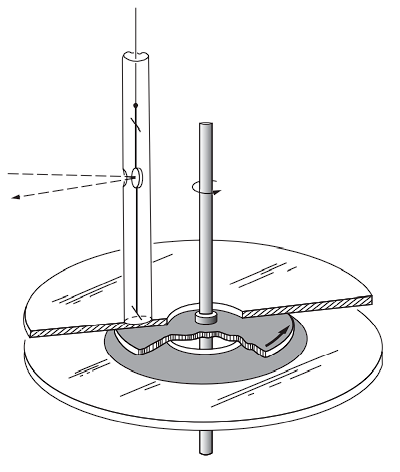
\includegraphics[width=0.8\textwidth]{rowland}
        \\{Figura 1: Principais partes do aparato de Rowland. As agulhas magnetizadas estão suspensas no tubo da esquerda}
        \label{fig:rowland}
    \end{figure}

    \begin{enumerate}
    	\item Encontre o campo magnético no eixo de rotação do disco.
    	\item Faça uma estimativa realista para os valores de carga, frequência de rotação, etc, para encontrar valores do campo magnético criado e sua variação quando a rotação é invertida. Compare com o campo magnético da Terra. Discuta as condições de realização do experimento.
    	\item Estime a direção, sentido e valor do campo magnético em pontos fora do eixo.
    	\item Discuta a diferença entre corrente de condução e corrente de convecção.
    \end{enumerate}

    \textbf{Referências bibliográficas estão no fim do documento.}

\newpage
\section {Campo magnético}
    \subsection{Análise quantitativa do experimento}
	A primeira coisa que devemos fazer é esquematizar o nosso problema de maneira mais quantitativa, portanto temos a seguinte figura:

	\begin{figure}[h]
        \centering
        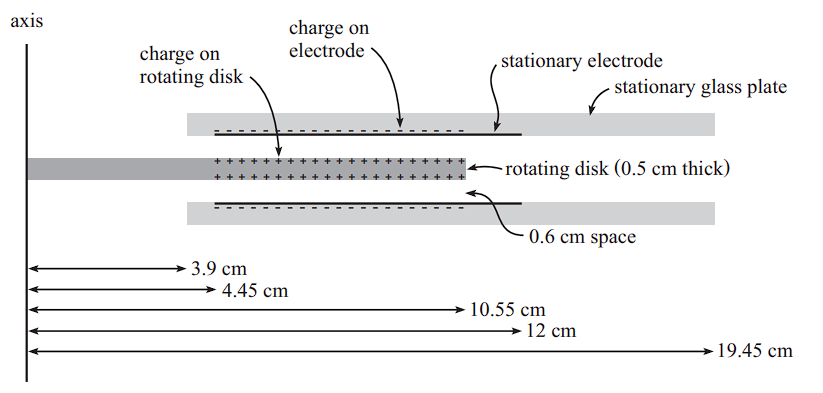
\includegraphics[width=0.9\textwidth]{rowland_diagram}
        \\{Figura 2: Esquema do experimento de Rowland com estimativas do experimento original}
        \label{fig:rowland_diagram}
    \end{figure}

    O nosso objetivo aqui é calcular o campo magnético aproximado logo acima do disco no experimento de Rowland.

    Vamos então calcular o campo elétrico na superfície do disco (imediatamente acima e abaixo do disco).
    \begin{equation} \label{e_field}
    	E = \frac{V}{d}
    \end{equation}

    A densidade de carga nas superfícies (em cima e em baixo do disco) será então
    \begin{equation} \label{q_density}
    	\sigma = \epsilon_0 E
    \end{equation}

    Sabendo que a quantidade de cargas em cada uma das pontas do disco (direita e esquerda), são determinadas pelas pontas do eletrodo de vidro, nós devemos trabalhar com um raio médio $\bar{r}$ para execução dos cálculos. Assim a velocidade média das cargas no disco será
    \begin{equation} \label{avg_v}
    	\bar{v} = 2\pi\bar{r}f
    \end{equation}

    Observe que essa é a velocidade no raio médio (meio do disco), e não a velocidade média das partículas. Mas para uma resultado grosseiro essa aprximação é suficiente. 

    Continuando, a densidade de corrente efetiva na superfície do disco é
    \begin{equation} \label{effective_density}
    	\mathcal{J} = \sigma\bar{v}
    \end{equation}

    O efeito combinado das duas placas de corrente (cada uma com densidade $\mathcal{J}$ na mesma direção), é para produzir um campo magnético horizontal $B = \mu_0\mathcal{J}$ tanto em cima quanto em baixo do disco. Escrevendo $B$ de maneira mais significativa temos
    \begin{equation} \label{b_field}
        B = \frac{2\pi\bar{r}f\mu_0\epsilon_0V}{d} = \frac{2\pi\bar{r}fV}{c^2d} = \frac{\bar{v}V}{c^2d}
    \end{equation}

    Substituindo os valores do diagrama e tomando $V = 10kV$ (que foi o utilizado por Rowland na maioria da iterações de seu experimento) obtemos os seguintes valores:
    $$
    E = \SI{1.67e6}{\volt\per\meter}
    $$$$
    \sigma = \SI{1.5e-5}{\coulomb\per\meter\squared}
    $$$$
    \bar{v} = \SI{28.7}{\meter\per\second}
    $$$$
    \mathcal{J} = \SI{4.3e-4}{\coulomb\per\second\per\meter}
    $$$$
    B = \SI{5.4e-10}{\tesla}
    $$

    Em nosso cálculos nós utilizamos os valores médios do raio e da velocidade, porém podemos obter um resultado mais preciso se dividissemos o nosso disco em vários aneis e integrassemos o resultado obtido para o disco completo. Isso foi o que Rowland fez.

    \subsection{Simplificação do experimento}
    Em uma esquematização mais simples do nosso problema podemos considerar um disco com densidade de cargas uniforme rotacionando com velocidade angular constante e desejamos calcular o campo magnético no eixo de rotação a uma certa distância do centro desse disco. Então nós devemos calcular quanto um anel a distância $x$ do centro contribui para nosso campo magnético
    \begin{equation}
    \begin{split}
        \delta q = 2\pi x\delta x \sigma \\
        \delta I = \frac{\delta q}{\delta t} = \frac{2\pi}{\delta t}x\delta x \sigma
    \end{split}
    \end{equation}

    Assim nosso diferencial de campo será
    \begin{equation}
        \delta B = \frac{\mu_0\delta I r^2}{2(x^2+d^2)^\frac{3}{2}}
    \end{equation}

    Integrando para o disco completo
    \begin{equation}
        \int \delta B = \int_{0}^{r} \frac{\mu_0\omega\sigma r^2 x}{2(x^2 + d^2)^\frac{3}{2}}\delta x
    \end{equation}

    Portanto
    \begin{equation} \label{simple_b_field}
        B = \frac{\mu_0\sigma\omega}{2}\left(\frac{r^2 + 2d^2}{\sqrt{r^2 + d^2}} - 2d \right)
    \end{equation}

    Assim obtemos um resultado mais simplificado porém muito significativo para nossa análise.
    \begin{figure}[h]
        \centering
        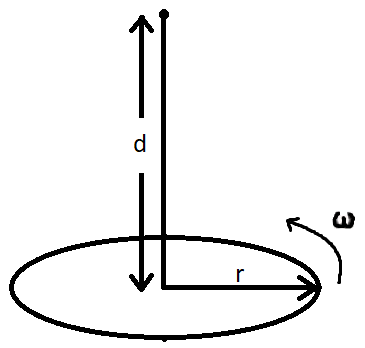
\includegraphics[width=0.4\textwidth]{simple}
        \\{Figura 3: Esquema mais simples do experimento de Rowland (densidade de carga uniforme $\sigma$ por todo disco)}
        \label{fig:simple}
    \end{figure}

    \subsection{Alteração da rotação}
    Como podemos perceber, a magnitude e a direção do nosso campo magnético dependem da direção de rotação do nosso disco. Na equação \ref{b_field} podemos ver que existe o vetor $\bar{v}$ e na equação \ref{simple_b_field} existe o $\omega$, que pode ser escrito em termos de um vetor $v$, que é a velocidade transversal do disco.

    Se a direção de rotação do nosso disco mudar, nosso campo vai ter mesma direção e mesma magnitude, porém sentido contrário, veja o seguinte esquema:

    \begin{figure}[h]
        \centering
        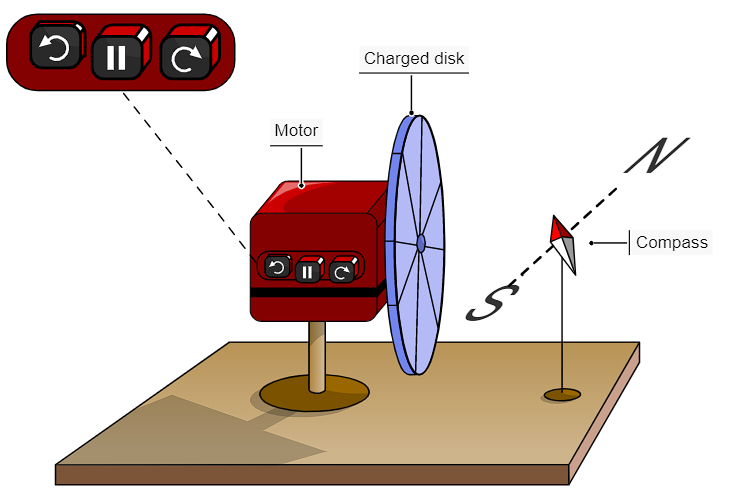
\includegraphics[width=0.6\textwidth]{counter_clockwise}
        \\{Figura 4: Disco de Rowland rotacionando no sentido anti-horário}
        \label{fig:counterclockwise}
    \end{figure}
    \begin{figure}[H]
        \centering
        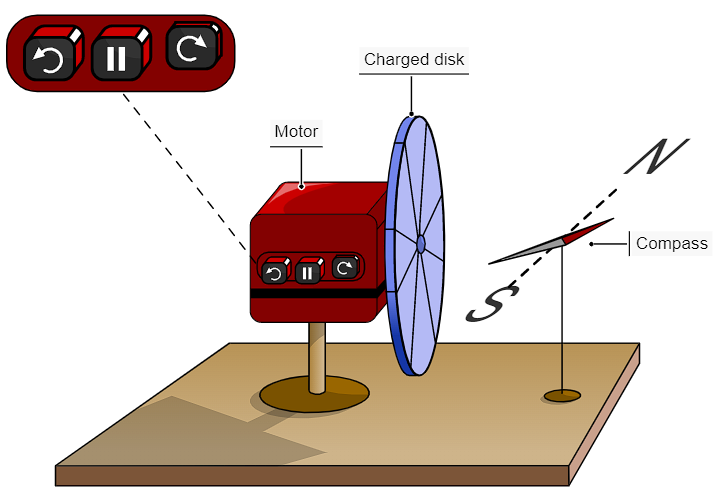
\includegraphics[width=0.6\textwidth]{clockwise}
        \\{Figura 5: Disco de Rowland rotacionando no sentido horário}
        \label{fig:counterclockwise}
    \end{figure}

    Nos esquemas ``N" e ``S" representam os polos magnéticos da terra.

    Perceba que nós podemos interpretar o nosso disco como um imã enquanto ele está rotacionando. Se ele está rotacionando na direção horária seu norte aponta para fora do disco, caso contrário, seu norte aponta para dentro do disco. Portanto o campo magnético fora do eixo do disco se comporta como um imã comum (de formato circular).
    \begin{figure}[h]
        \centering
        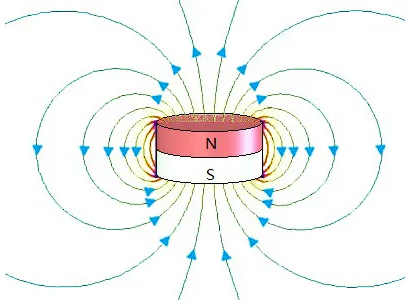
\includegraphics[width=0.6\textwidth]{disc}
        \\{Figura 6: Imã em formato de disco}
        \label{fig:counterclockwise}
    \end{figure}

\newpage
\section{Correntes de convecção e de condução}
    A definição de corrente é a variação de carga em um determinado paríodo de tempo. Como essa carga está se movimentando é o que vai definir se essa corrente é de convecção ou de condução.

    Correntes de convecção são cargas que estão se movimentando a partir de uma força que não seja gerada por um campo magnético, ou seja, essas cargas não são guiadas (conduzidas) por um campo magnético. Um bom exemplo que ocorre no mundo real é a movimentação de ondas que carregam elétrons livres se movimentando pelas atmosfera com a força do vento.

    Por outro lado, correntes de condução são aquelas cujo suas cargas estão sob o efeito de um capo elétrico, como pro exemplo em um fio de cobre (condutor) ligado a uma bateria. Essas são definitivamente mais comuns no mundo real, até porquê qualquer circuito elétrico/eletrônico é um exemplo de correntes de condução.

\newpage
\section{Referências}
    \subsection{Figuras}
    Figura 1: Purcell, Edward M. \& Morin, David J., Electricity and Magnetism, Cambridge University Press (3rd edition, 2013) (1st edition, vol. 2 da Coleção de Física de Berkeley, 1963).

    Figuras 2 e 6: Google Images

    Figura 3: Autoral

    
    Figuras 4 e 5: \href{https://www.edumedia-sciences.com/en/media/108-rowlands-disk}{Rowland's Disk simulation} 

    \subsection{Referências bibliográficas}
    Mazur, Eric, Principles \& Practice of Physics, Pearson Education (2015)

    Bauer, Westfall \& Dias, Física para Universitários, McGraw-Hill  (1a ed., 2012)

    Halliday, Resnick \& Walker, Fundamentos de Física, LTC (10a ed., 2012).

    Jewett \& Serway, Física para cientistas e engenheiros, Cengage (9a ed. (EUA), 2a ed (Brasil), 2018).

    Purcell, Edward M. \& Morin, David J., Electricity and Magnetism, Cambridge University Press (3rd edition, 2013) (1st edition, vol. 2 da Coleção de Física de Berkeley, 1963).

    Nussenzveig, H.M., Eletromagnetismo, Curso de Física Básica, vol. 3, Ed. Edgard Blücher, (1997).

    \href{https://en.wikipedia.org/wiki/Electric_current}{Electric Current (Wikipedia)}

\end{document}
